\chapter{Reinforcement Learning} 
Dieses Kapitel dient dazu, die Grundlagen von Reinforcement Learning zu erläutern. Dabei wird besonderer Fokus auf die Terminologie sowie auf grundlegende Konzepte und Algorithmen gelegt. 
Im Gegensatz zu anderen Machine-Learning-Gebieten wird beim Reinforcement Learning nicht zwingend mit verfügbaren Daten gearbeitet. Die benötigten Informationen werden durch ‹Trial-and-Error› generiert. Ein sogenannter Agent führt in einer Simulationsumgebung, dem Environment, Handlungen aus. Diese Handlungen werden Actions genannt. 
 

 \begin{figure}[ht]
  \centering
  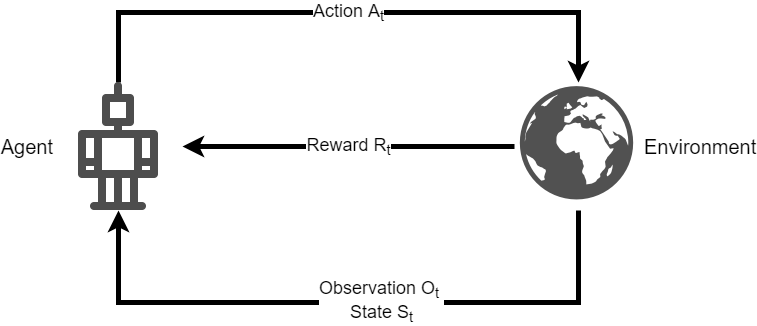
\includegraphics[height=4.5cm]{img/RL_Agent_Env.png}
  \label{rl_draw}
  \caption{RL-Agent und Environment}
\end{figure}

Nach jeder Action erhält der Agent einen Reward und eine Observation. Der Reward informiert den Agent, wie gut seine Action war. Dabei kann der Reward sowohl positiv als auch negativ sein. Die Wahl des Rewards hängt vom Environment und dem Task ab. Er könnte dem gewonnenen Score in einem Spiel entsprechen, einem Börsen-Kurs oder einem vordefinierten Wert für gewisse Umstände im Environment. Daneben erhält der Agent auch eine Observation. Die Observation enthält Informationen aus dem State des Environments. In einer perfekten Welt umfasst die Observation den gesamten Space des Environments. In diesem Fall würde der State im Agent dem des Environments entsprechen. Wenn in Reinforcement Learning vom State gesprochen wird, ist im Normalfall die Rede vom internen State des Agents. Das Ziel des Agents ist es, den gesamten Reward zu maximieren.

\section{Markov-Prozess}
Reinforcement Learning setzt voraus, dass Entscheidungen in einem Environment nach dem Markov-Decision-Process (MDP) getroffen werden. Jedes Environment handelt nach einem MDP. In den folgenden Kapiteln werden die Bestandteile, welche einen MDP ausmachen, beschrieben. Dadurch soll ein Verständnis aufgebaut werden, wie ein MDP gelöst werden kann. Ein MDP setzt die Markov-Eigenschaft voraus. Diese Eigenschafft ist erfüllt, wenn in einem stochastischen Prozess die Wahrscheinlichkeitsverteilung für zukünftige States nur vom aktuellen State abhängig ist und nicht von der Vergangenheit. Jede Umgebung kann grundsätzlich als MDP definiert werden; dazu müssen nur genügend Informationen im State vorhanden sein, welcher unter Umständen auch die Vergangenheit selbst beinhaltet.

\begin{equation}
\mathbb{P}[S_{t+1}\ |\ S_t]=\ \mathbb{P}[S_{t+1}\ |\ S_1,\ \ldots,\ S_t]
\end{equation}

Aufbauend auf dieser Eigenschaft entsteht ein Markov-Prozess. Dieser Prozess ist eine Sequenz von zufälligen States, welche die Markov-Eigenschaft haben. Der Markov-Prozess ist ein Tupel aus $\mathcal{S}$, dem State-Space, einer endlichen Anzahl möglicher States und $\mathcal{P}$, der Übergangsmatrix, welche für jeden State-Übergang die Wahrscheinlichkeit beschreibt. Anhand dieser Tupel kann eine Kopie des Environments erstellt werden, welche genau gleich auf die States reagiert.


 \begin{figure}[ht]
 \centering
  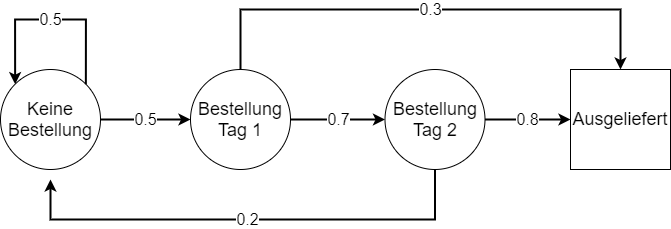
\includegraphics[height=5cm]{img/Markov_Prozess_Ext.png}
  \caption{Markov-Prozess}
  \label{mp_draw}
\end{figure}


Das Beispiel in Abbildung \ref{mp_draw} zeigt einen solchen Markov-Prozess auf. Im Status «Keine Bestellung» besteht eine Übergangswahrscheinlichkeit von 50 Prozent, dass eine neue Stellung eintrifft. Ist eine Bestellung eingetroffen, besteht die Wahrscheinlichkeit von 30 Prozent, dass der Artikel bereits vorhanden ist und direkt ausgeliefert wird. Wurde die Bestellung nicht ausgeliefert, so besteht am nächsten Tag erneut eine Wahrscheinlichkeit, dass der Artikel nun vorhanden ist und ausgeliefert wird. Ist das nicht der Fall, annulliert in diesem Beispiel der Kunde die Bestellung.

\section{Markov Reward Process}
Der Markov-Reward-Process (MRP) baut auf dem Markov-Prozess auf und fügt eine Wertung der Übergänge hinzu. Der MRP wird durch die Tupel $\langle S,P,R,\gamma \rangle$ beschrieben. Dabei steht $\mathcal{R}$ für die Reward-Funktion; diese beschreibt, welcher State welchen Reward erhält. 

 \begin{figure}[ht]
  \centering
  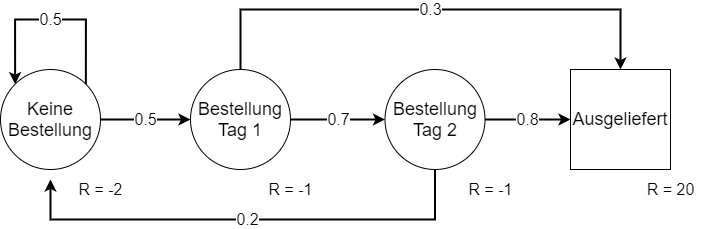
\includegraphics[height=5cm]{img/Markov_Reward_Prozess.png}
  \caption{Markov-Reward-Process}
  \label{mrp_draw}
\end{figure}

Der Discount-Factor $\gamma$ beschreibt, wie stark zukünftige Rewards gewichtet werden. Ein Discount-Factor von 1 beachtet alle zukünftigen Rewards und ein Discount-Factor von 0 betrachtet nur den aktuellen Reward. Das Ziel in einem MRP ist es, den Return $G_t$, den gesamten diskontierten Reward eines Zeitschritts $t$, zu maximieren.

\begin{equation}
    G_t=R_{t+1}+{\gamma R}_{t+2}+{\gamma^2R}_{t+3}+...\ =\sum_{k=0}^{\infty}{\gamma^kR}_{t+k+1}
\end{equation}

\newpage
Um den Return genauer zu veranschaulichen, folgen nun einige mögliche Sequenzen des MRPs aus Abbildung \ref{mrp_draw}. Es wird ein Discount-Factor von 0.5 verwendet und die Sequenzen starten beim State «Keine Bestellung».



\begin{align}
    &\boldsymbol{KB\xrightarrow{}BT1\xrightarrow{}A}\nonumber\\
    &v=-2+(-1\ast\frac{1}{2})+(20\ast\frac{1}{4})\ =2.5\\ \nonumber\\
    &\boldsymbol{KB\xrightarrow{}BT1\xrightarrow{}BT2\xrightarrow{}A}\nonumber\\
    &v=-2+(-1\ast\frac{1}{2})+(-1\ast\frac{1}{4})+(20\ast\frac{1}{8})\ =-0.25\\ \nonumber\\
    &\boldsymbol{KB\xrightarrow{}BT1\xrightarrow{}BT2\xrightarrow{}KB\xrightarrow{}KB\xrightarrow{}BT1\xrightarrow{}A}\nonumber\\
    &v=-2+(-1\ast\frac{1}{2})+(-1\ast\frac{1}{4})+(-2\ast\frac{1}{8})+(-2\ast\frac{1}{16})+(-1\ast\frac{1}{32})+(20\ast\frac{1}{64}) \nonumber\\
    &v=-\frac{91}{32}\approx-2.84
\end{align}



\section{Bellman-Expectation-Equation}
Die Value-Function wertet einen gegebenen State aus. Dabei wird der erwartete Return für den entsprechenden State berechnet. 




\begin{align}
&v(s)\ =\ \mathbb{E}\ [G_t\ |{\ S}_t=s] \nonumber\\
&v(s)\ =\ \mathbb{E}\ [R_{t+1}+{\gamma G}_{t+1}\ |{\ S}_t=s] \nonumber\\
&v(s)\ =\ \mathbb{E}\ [R_{t+1}+{\gamma v(S}_{t+1})\ |{\ S}_t=s] \label{bellman-exp-equa}
\end{align}


Bei der Value-Function handelt es sich um eine rekursive Gleichung, wobei der Wert der aktuellen States aus dem zu erwartenden Reward und dem diskontierten Wert des folgenden States besteht. Dies entspricht der Bellman-Expectation-Equation; diese kann auch als Matrixrepräsentation dargestellt werden.
\begin{equation}
  v=\mathcal{R}+\gamma\mathcal{P}v
\end{equation}

\begin{equation}
\left[\begin{matrix}v(1)\\\vdots\\v(n)\\\end{matrix}\right]\ =\left[\begin{matrix}\mathcal{R}_1\\\vdots\\\mathcal{R}_n\\\end{matrix}\right]\left[\begin{matrix}\mathcal{P}_{11}&\cdots&\mathcal{P}_{1n}\\\vdots&\ddots&\vdots\\\mathcal{P}_{n1}&\cdots&\mathcal{P}_{nn}\\\end{matrix}\right]\left[\begin{matrix}v(1)\\\vdots\\v(n)\\\end{matrix}\right]
\end{equation}


Diese lineare Gleichung kann direkt gelöst werden:
\begin{align}
 v&=\mathcal{R}+\gamma\mathcal{P}v \nonumber\\
\left(I-\gamma\mathcal{P}\right)\ v&=\mathcal{R} \nonumber\\
v&=\left(I-\gamma\mathcal{P}\right)^{-1}\ \mathcal{R} \label{solve-lin-equa}
\end{align}



Dabei ist zu beachten, dass diese Variante nur für kleine MRPs geeignet ist, da die Zeitkomplexität für diese Berechnung $0(n^3)$ beträgt, wobei n für die Anzahl States steht. Für grössere MRPs gibt es erweiterte Methoden, welche noch in den folgenden Kapiteln erläutert werden. Nun kann diese Formel am MRP aus dem vorherigen Beispiel angewendet werden. In diesem Beispiel wird ein Discount-Factor von 1 verwendet, womit alle zukünftigen Returns berücksichtigt werden.

\begin{equation}
  \left(\left[\begin{matrix}\begin{matrix}1&0\\0&1\\\end{matrix}&\begin{matrix}0&0\\0&0\\\end{matrix}\\\begin{matrix}0&0\\0&0\\\end{matrix}&\begin{matrix}1&0\\0&1\\\end{matrix}\\\end{matrix}\right]-1\left[\begin{matrix}\begin{matrix}0.5&0.5\\0&0\\\end{matrix}&\begin{matrix}0&0\\0.7&0.3\\\end{matrix}\\\begin{matrix}0.2&0\\0&0\\\end{matrix}&\begin{matrix}0&0.8\\0&0\\\end{matrix}\\\end{matrix}\right]\right)^{-1}\left[\begin{matrix}\begin{matrix}-2\\-1\\\end{matrix}\\\begin{matrix}-1\\20\\\end{matrix}\\\end{matrix}\right]=\left[\begin{matrix}\begin{matrix}13.37\\17.37\\\end{matrix}\\\begin{matrix}17.67\\20\\\end{matrix}\\\end{matrix}\right]  
\end{equation}


In der folgenden Abbildung ist der MRP mit den Values der jeweiligen States ersichtlich.
 \begin{figure}[h]
  \centering
  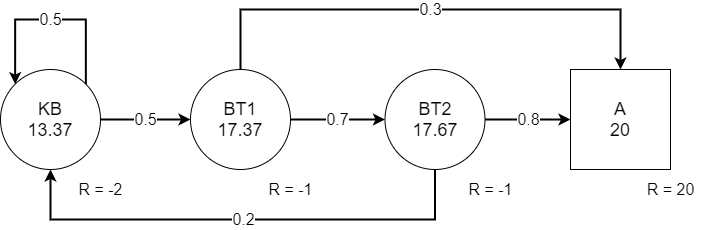
\includegraphics[width=\textwidth]{img/Bellman_Expectation_Equation.png}
  \caption{MRP mit Values}
\end{figure}

Ob diese Values stimmen, kann nun problemlos mit einem vorausschauenden Schritt in einem beliebigen State überprüft werden. Die Zahlen wurden auf zwei Kommastellen gerundet.


\begin{align}
&v(BT2) = \mathbb{E} [G_t |{ S}_t=s] \nonumber\\
\begin{split}
v(BT2) =R_{t+1}+ \gamma v(KB)\ast P(KB)+ \gamma v(BT1)\ast P(BT1) \\
+ \gamma v(BT2)\ast P(BT2)+\gamma v(A)\ast P(A) 
\end{split}\nonumber\\ 
&v(BT2) =-1+ 13.37\ast0.2+ 17.37\ast0+ 17.67\ast0+20\ast0.8 \nonumber\\
&v(BT2) = 17.67 \label{calculate-mrp}
\end{align}


		
\section{Markov-Decision-Process}
Der Markov-Decision-Process (MDP) erweitert den MRP um $\mathcal{A}$, eine endliche Anzahl möglicher Actions. Somit wird der MDP mit dem folgenden Tupel definiert $\langle S,A,P,R,\gamma \rangle$.  Dabei wird die Übergangsmatrix $\mathcal{P}$ mit der jeweiligen Action erweitert und beschreibt somit die Wahrscheinlichkeit der State-Action-Übergänge. Auch die Reward-Funktion $\mathcal{R}$ benötigt zusätzlich eine Action, um den Reward zu berechnen. Da nun die State-Übergänge durch Actions beeinflusst werden, muss die Value-Function angepasst werden. Die Value-Function wird nun so angepasst, dass sie einer Strategie, einer sogenannten Policy $\pi$, folgt. Eine solche Policy beschreibt für einen State S, mit welcher Wahrscheinlichkeit die möglichen Actions gewählt werden. Die Value-Function $v_\pi(S)$ beschreibt den Wert eines States – vorausgesetzt, die zukünftigen Actions werden nach der Policy $\pi$ gewählt. 

\begin{equation}
v_\pi(S)\ ={\ \mathbb{E}}_\pi\ [R_{t+1}+{\gamma v_\pi(S}_{t+1})\ |{\ S}_t=s]
\end{equation}

Um einen MDP zu lösen und eine optimale Policy zu finden, muss unterschieden werden, ob das Model bekannt ist, welches das Environment beschriebt – also die kompletten Tupel, die den MDP beschreiben. Oft sind nicht alle Dynamiken eines Environments bekannt oder die Menge an zu verarbeitenden Informationen ist nicht mehr geeignet.

In Abbildung \ref{fig:mdp} wird erneut das Lagerbeispiel verwendet. Die States wurden zudem mit der Information erweitert, ob ein Artikel auf Lager ist oder nicht. Ausserdem verfügt nun der Agent über drei verschiedene Actions: A1 – \emph{Warten}, A2 – \emph{Beim Lieferanten bestellen} und A3 – \emph{Ausliefern}. Die drei Kreuzungen zwischen den States stellen die probabilistischen Ausgänge aus den jeweiligen Actions dar. Falls in diesem Beispiel ein Artikel beim Lieferanten bestellt wird, so ist dieser garantiert am nächsten Tag da. Die Wahrscheinlichkeit, dass am nächsten Tag eine neue Bestellung von einem Kunden eintrifft, ist nur 50 Prozent.

 \begin{figure}[h]
  \centering
  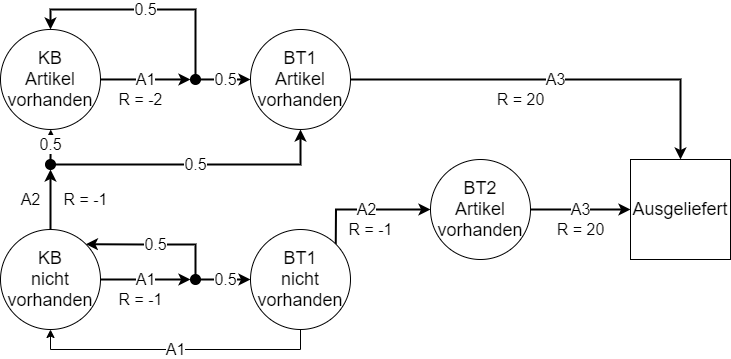
\includegraphics[width=\textwidth]{img/Markov_Decision_Prozess.png}
  \caption{Markov-Decision-Process}
  \label{fig:mdp}
\end{figure}




\section{Bellman-Optimality-Equation}
Anders als bei der Bellman-Expectation-Equation, die bereits zum Evaluieren der Value-Function einer bestimmten Policy benötigt wird, ist die Bellman-Optimality-Equation keine lineare Gleichung. Wenn in der Literatur von der Bellman-Equation die Rede ist und nicht weiter spezifiziert wird, betrifft es meistens die Bellman-Optimality-Equation. Das Ziel dieser Gleichung ist es nicht, den Wert eines States bei einer definierten Policy $\pi$ zu evaluieren, sondern eine optimale Policy $\ast$ zu finden. 

\begin{align}
&v_\ast(s)\ =\max_\pi{v_\pi}(s) \nonumber\\
&v_\ast(s)\ =\max_a{\mathcal{R}(s,a)}+\gamma\sum_{S^\prime}{\mathcal{P}(s,a,s^\prime)}v_\ast(s^\prime) \label{bellman-opt-equa}
\end{align}


\newpage
Dabei wird bei der optimalen State-Value-Function nicht die optimale Policy gesucht, sondern der maximal mögliche Reward, welcher der Agent aus einem Environment bekommen kann. Im Beispiel des MDP würden bei einem Discount-Factor von 1 folgende Values errechnet (Anhang \ref{appendix:state-values}):

\begin{figure}[ht]
  \centering
  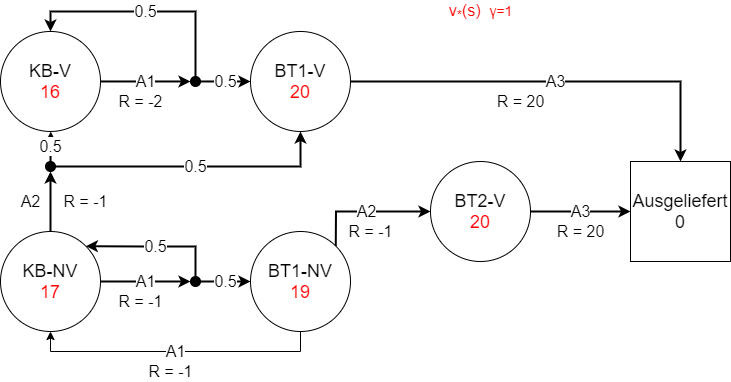
\includegraphics[width=\textwidth]{img/MDP_State-Value_Function.png}
  \caption{MDP-State-Value-Function}
    \label{fig:mdp-value}
\end{figure}
Um die optimale Policy zu finden, welche den MDP komplett löst, wird die optimale Action-Value Function benötigt.
\begin{align}
&q_\ast\left(s,a\right)=\max_\pi{q_\pi}\left(s,a\right) \nonumber\\
&q_\ast(s,a)\ =\mathcal{R}(s,a)+\gamma\sum_{S^\prime}{\mathcal{P}(s,a,s^\prime)}{max\ {q_\ast}_{a^\prime}(s^\prime,a^\prime)} \label{bellman-opt-equa-q}
\end{align}

\newpage
Die optimale Action-State-Function sagt für einen State und eine Action aus, welches der maximale zukünftige Reward für die aktuelle Situation ist. Die entsprechenden Q-Values für diese optimale Policy wurde im Anhang \ref{appendix:action-values} berechnet.
 \begin{figure}[H]
  \centering
  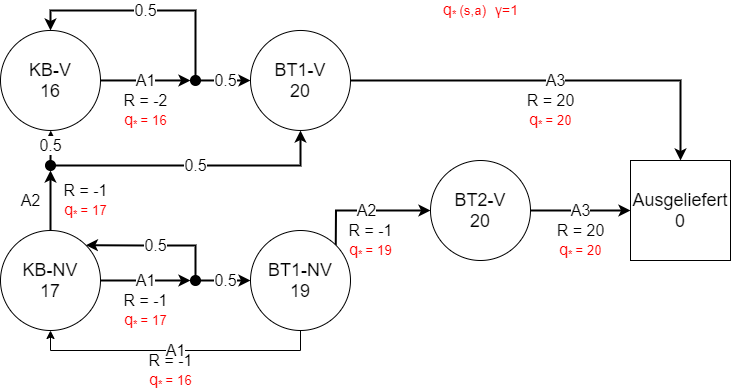
\includegraphics[width=\textwidth]{img/MDP_Action-Value_Function.png}
  \caption{MDP-Action-Value-Function}
      \label{fig:mdp-action-value}
\end{figure}

Betrachtet man in diesem Beispiel (Abbildung \ref{fig:mdp-action-value}) den Start-State «KB-NV», so wird nun klar, dass der maximal mögliche Reward 17 ist, egal ob die Action A1 – \emph{Warten} oder die Action A2 – \emph{Beim Lieferanten bestellen} ausgeführt wird. Mit diesen Q-Values der optimalen Policy können nun die Actions in diesem MDP immer optimal gewählt werden. Ein MDP hat zwingend mindestens eine deterministisch optimale Policy.


\section{Model-free Prediction}
Bei der Model-free Prediction kennt der Agent das Model des MDP nicht. Der Agent sammelt Informationen über das Environment und versucht so, seine aktuelle Policy zu evaluieren. Dazu gibt es diverse Methoden, welche aber im Grundsatz auf den folgenden beiden Methoden aufbauen.
\subsection{Monte-Carlo-Learning}
Die Monte-Carlo(MC)-Methode evaluiert eine Policy anhand der Erfahrung ganzer Episoden. Eine Episode stellt eine Sequenz an Actions dar, die in einem Environment durchgeführt werden. Diese Durchführung von Actions geschieht so lange, bis ein Abbruchkriterium erreicht ist und somit die Episode beendet wurde. Der Agent führt eine bestimmte Sequenz lang Actions nach der Policy durch, bis die Episode beendet wird. Dabei wird eine Anzahl an Episoden festgelegt, die der Agent durchläuft. Bei dieser Methode benötigt der Agent zwingend die kompletten Episoden zum Evaluieren. Der Agent durchläuft dabei die Episoden, nimmt den jeweiligen Return und berechnet den durchschnittlichen Return für alle Episoden. Der dabei berechnete empirische Return konvergiert mit steigender Anzahl der Episoden gegen den zu erwartenden Return. Somit nähert sich auch die Value-Function der tatsächlichen Value-Function an.
\subsection{Temporal-Difference-Learning}
Im Gegensatz zur MC-Methode evaluiert die Temporal-Difference(TD)-Methode eine Policy nicht mit der Erfahrung aus einer kompletten Episode, sondern aus einer Schätzung, welche aus einer Sequenz von Actions durchgeführt wurde. Es wird eine bestimmte Anzahl $n$ Actions durchgeführt, mit welchen anschliessend eine Schätzung für den Return durchgeführt wird. Daraufhin wird nach den nächsten n Actions die Schätzung der Values mit der neuen Schätzung des Returns aktualisiert. Dieses Vorgehen wird Bootstrapping genannt, da eine Schätzung aufgrund einer anderen Schätzung durchgeführt wird.

 \begin{figure}[ht]
  \centering
  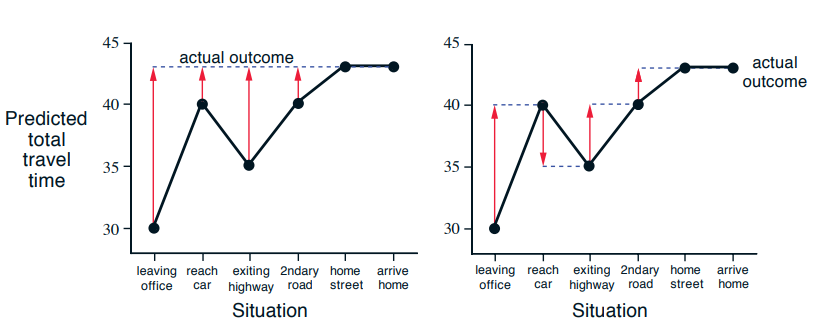
\includegraphics[width=\textwidth]{img/diff_mc_td.png}
  \caption{Unterschied MC \& TD \cite{td-mc}}
      \label{fig:diff-mc-td}
\end{figure} 


\newpage
\section{Model-free Control}
Ist das Model eines MDPs bekannt und der Agent kennt die Übergangswahrscheinlichkeiten sowie die Reward-Funktion des MDPs, so kann mittels Dynamic-Programming und Policy-Iteration die optimale Policy erlernt werden. Oft ist in der Realität bei Problemstellungen, in denen Reinforcement Learning angewendet wird, kein Model bekannt, welches den genauen MDP beschreibt. Daher muss der Agent wie in der Model-free Prediction mithilfe gemachter Erfahrungen die aktuell angewendete Policy evaluieren und verbessern. Zur Verbesserung einer Policy ist ein gewisses Mass an Exploration nötig. Ein Agent, welcher nicht exploriert, sondern nur exploitiert, wählt die aus seiner aktuellen Policy beste Action. Stellt man sich ein minimales Beispiel vor, in dem eine Action im aktuellen State einen Reward von 2 ergibt und die andere einen Reward von 10, wird – sofern die erwarteten Returns mit 0 initialisiert wurden und somit beide einen gleichen erwarteten Return haben – eine zufällige erste Action gewählt. Bei der Wahl einer Action, welche einen Reward von 2 ergibt, wird ohne Exploration nie eine andere Action ausprobiert und der Reward von 10 würde somit nie erreicht werden. 
\subsection{Epsilon-greedy Exploration}
Die Epsilon-greedy Exploration ist eine oft verwendete Methode, um sicherzustellen, dass der Agent neue Actions ausprobiert und somit das ganze Environment kennenlernt. So kann er die bestmögliche Policy finden. Dabei wird ein Wert $\epsilon$ (Epsilon) zwischen 0 und 1 festgelegt. Vor jeder Action wird mit der Wahrscheinlichkeit 1 - $\epsilon$ die beste Action, die Greedy Action ausgeführt. Mit der Wahrscheinlichkeit $\epsilon$ wird eine zufällige Action ausgeführt. Würden unendlich viele Schritte durchgeführt, so würde jedes State-Action-Paar unendlich oft besucht werden. Somit kann ausgeschlossen werden, dass eine bestimmte Policy nicht entdeckt wird.

\begin{equation}
   \pi(a|s)
\left\{\begin{matrix}
 1-\epsilon,&  \underset{a\in A} {\mathrm{argmax}} ~Q(s,a)\\ 
 \epsilon,& random(a)
\end{matrix}\right. 
\end{equation}

Ein Nachteil bei der Epsilon-greedy Exploration ist, dass die Policy nie wirklich mit der optimalen Policy konvergiert, da weiterhin zufällig Actions ausgeführt werden. Eine Möglichkeit, dem entgegenzuwirken, besteht darin, $\epsilon$ über die Zeit zu verkleinern.




\subsection{Sarsa}
Der Sarsa-Algorithmus \cite{rummery1994line} basiert auf dem Prinzip der TD. Dabei wird in einem State-Action-Paar gestartet. Der Agent erhält ein Reward und erreicht einen neuen State. Nun nimmt der Agent seine Schätzung für das folgende State-Action-Paar der Policy; dieser diskontierte Q-Value zusammen mit dem Reward muss laut der Bellman-Equation dem vorherigen Q-Value entsprechen. Der Ausgangs-Q-Value $Q\left(S,A\right)$ wird anhand der Lernrate $\alpha$ in Richtung TD-Target korrigiert (\ref{sarsa_eq}). Die Differenz zwischen TD-Target und dem Ausgangs-Q-Value ist der TD-Error; dieser muss bei einer Greedy Policy konvergieren, sonst wurde keine optimale Policy gefunden. 

 \begin{figure}[ht]
  \centering
  
\includegraphics[height=3cm]{img/SARSA (1).png}
  \caption{Sarsa-Update}
      \label{fig:sarsa-update}
\end{figure} 

\begin{align}
&Q\left(S,A\right)\gets Q\left(S,A\right)+\alpha\left(R+\gamma Q\left(S^\prime,A^\prime\right)-Q\left(S,A\right)\right) \nonumber\\
&Q\left(S,A\right)\gets Q\left(S,A\right)+\alpha\left(TDTarget-Q\left(S,A\right)\right) \nonumber\\
&Q\left(S,A\right)\gets Q\left(S,A\right)+\alpha\left(TDError\right) \label{sarsa_eq}
\end{align}




\begin{algorithm}
\begin{algorithmic}[1]
\State{Algorithm parameters: step size $\alpha \in$ (0, 1), small $\epsilon$ > 0}
\State{Initialize  $Q(s,a)$, for all $s\in S^+,a\in A(s)$, arbitrarily except that $Q(terminal)$=0}
\Repeat { for each episode}
\State{Initialize $S$}
\State{Choose $A$ from $S$ using policy derived from $Q$ (e.g., $\epsilon$-greedy)}
  \Repeat{ for each step of episode}
    \State {Take action $A$, observe $R$, $S'$}
    \State {Choose $A'$ from $S'$ using policy derived from $Q'$ (e.g., $\epsilon$-greedy)}
    \State {$Q(S,A)\gets Q(S,A)+ \alpha [R+ \gamma Q(S',A') -Q(S,A)]$}
    \State {$S\gets S'; A \gets A';$}
    \Until{$S$ is terminal}
\end{algorithmic}
\caption{Sarsa-Algorithmus \cite{sutton_reinforcement_2018} Chapter 6}
\end{algorithm}




\subsection{Q-Learning}
Im Gegensatz zu Sarsa ist Q-Learning \cite{dayan1992q, watkins1989learning} ein Off-Policy-Algorithmus. Das bedeutet, der Agent wählt zwar – wie bei Sarsa – eine Action nach der Epsilon-greedy Policy, nimmt aber für die Schätzung die Action nach der Greedy Policy. Dieses Vorgehen entspricht dem Prinzip der Bellman-Optimality-Equation.

 \begin{figure}[ht]
  \centering
  
\includegraphics[height=3cm]{img/Q-Learning.png}
  \caption{Q-Learning-Update}
      \label{fig:q-update}
\end{figure} 








\begin{equation}
    Q\left(S,A\right)\gets Q\left(S,A\right)+\alpha\left(R+\gamma\max_{a^\prime}
{Q\left(S^\prime,a^\prime\right)}-Q\left(S,A\right)\right)
\end{equation}


\begin{algorithm}
\begin{algorithmic}[1]
\State{Algorithm parameters: step size $\alpha \in$ (0, 1), small $\epsilon$ > 0}
\State{Initialize  $Q(s,a)$, for all $s\in S^+,a\in A(s)$, arbitrarily except that $Q(terminal)$=0}
\Repeat { for each episode}
\State{Initialize $S$}
  \Repeat{ for each step of episode}
    \State{Choose $A$ from $S$ using policy derived from $Q$ (e.g., $\epsilon$-greedy)}
    \State {Take action $A$, observe $R$, $S'$}
    \State {$Q(S,A)\gets Q(S,A)+ \alpha [R+ \gamma max_a Q(S',a) -Q(S,A)]$}
    \State {$S\gets S'$}
    \Until{$S$ is terminal}
\end{algorithmic}
\caption{Q-Learning-Algorithmus \cite{sutton_reinforcement_2018} Chapter 6}
\end{algorithm} 